% vim: set foldmethod=marker conceallevel=2:
%! TEX root = preprint.tex

% Introduction {{{1

The Van der Waals (vdW) interactions originate from nonlocal correlations in the quantum motion of electrons, and give rise to a wide spectrum of physical phenomena, ranging from attraction between two atoms~\citep{LondonZP30} to the macroscopic Casimir effect~\citep{JaffePRD05}.
They dictate thermodynamic properties of many molecular solids, layered and nanostructured materials, and biological compounds, and govern processes such as molecular adsorption and self-assembly, including most biological processes.
As a result, vdW interactions have been, and are increasingly so, one of the prime targets of material modeling, which has led to a plethora of approaches that either treat vdW forces on the same footing as the rest of electron correlation or model them explicitly~\citep{KlimesJCP12,GrimmeCR16,HermannCR17}.
These include quantum Monte--Carlo~\citep{AmbrosettiJPCL14} (QMC), coupled clusters~\citep{YangS14}, random-phase approximation~\citep{LuPRL09}, nonlocal density functionals~\citep{DionPRL04,VydrovPRL09}, and coarse-grained approaches, which range from pairwise~\citep{GrimmeJCC04,BeckeJCP07,TkatchenkoPRL09} to many-body models~\citep{TkatchenkoPRL12,SilvestrelliJCP13}.
From theoretical perspective, this status quo is undesirable, because different models often give disparate pictures of the nature of vdW forces, which leads to incoherent understanding of vdW interactions in molecules and materials.
From practical perspective, the three main characteristics of a method are its applicability, accuracy, and computational efficiency, and so far, no single method has satisfied all three requirements with respect to vdW forces to such a degree, that it would be reliably applicable to all the relevant types of materials.
For instance, QMC and coupled clusters are limited by computational efficiency, pairwise approaches lack in accuracy for nanostructured and supramolecular compounds, and coarse-grained models have qualitative problems with description of ionic and hybrid metal-organic systems.

In this Letter, we present a unified density-functional model of vdW interactions that combines ingredients from nonlocal functionals and coarse-grained models, inheriting broad applicability of the former and good accuracy of the latter, while retaining the computational efficiency of both.
We integrate the polarizability functional of \citet{VydrovPRA10} (VV), normalization to reference free-atom vdW parameters coined by the vdW model of \citet{TkatchenkoPRL09} (TS), the idea of normalization to jellium via a zero-gradient limit from the VV10 nonlocal functional~\citep{VydrovJCP10a}, and the Hamiltonian form of the many-body dispersion (MBD) model~\citep{TkatchenkoJCP13}.
Compared to the range-separated self-consistently screened (rsSCS) variant of MBD~\citep{AmbrosettiJCP14}, the use of the VV polarizability functional in the new model enables consistent treatment of ionic compounds, normalization to free-atom reference values balances the accuracy of the VV polarizability across the periodic table, while normalization to jellium enables effective modeling of adsorption on metallic surfaces~\citep{RuizPRL12}.
Furthermore, the VV functional---unlike approaches based on Hirshfeld volumes---is able to capture short-range many-body polarization effects, so that the short-range screening of atomic polarizabilities is not needed in the new model, reducing the overall computational cost by an order of magnitude compared to MBD@rsSCS\@.
In our consideration, a similar level of empiricism is involved in the construction of the new model compared to MBD@rsSCS\@.
On one hand we remove the need for tabulated reference vdW radii and for the short-range screening, on the other we introduce a mechanism to avoid double-counting of electron correlation in near-uniform density regions that involves some empirical choices.
However, these choices are motivated theoretically, and justified qualitatively without resorting to empirical arguments.
We demonstrate on a series of benchmark calculations that our new model enables for the first time consistent treatment of vdW interactions in covalent, ionic, and hybrid metal-organic interfaces by a single method, while achieving the accuracy of best existing approaches for each of these material types.

% Model {{{1

% Coarse graining {{{2

The central proposition of the new model, dubbed MBD-NL, is to parameterize the Hamiltonian of the MBD model with the polarizability density from the VV10 nonlocal functional.
In general, each vdW model consists of two main ingredients: a model for the noninteracting electrodynamic response and the model for long-range coupling of this response.
The shortcomings of many existing vdW approaches in description of ionic compounds and hybrid interfaces do not originate from the model for the coupling, but rather from the model for the response.
Its improvement is the main focus of this work.
In the case of coarse-grained models, such as MBD, the model for the response translates into a model for static polarizabilities $\alpha_{0,i}$ and $C_{6,ii}$ coefficients of the interacting fragments (usually atoms).
In MBD-NL, we parametrize the response of atoms by coarse-graining the VV polarizability density to Hirshfeld fragments~\citep{HirshfeldTCA77,SatoJCP09,SatoJCP10}.
The VV polarizability functional is a semilocal functional of the electron density $n(\mathbf r)$, which models local isotropic dynamic polarizability density,
\begin{equation}
   \alpha^\text{VV}[n](\mathbf r,\mathrm iu)=\frac{n(\mathbf r)}{\frac{4\pi}3n(\mathbf r)+C\frac{{|\boldsymbol\nabla n(\mathbf r)|}^4}{n{(\mathbf r)}^4}+u^2}
   \label{eq:vv-functional}
\end{equation}
where $\mathrm iu$ is imaginary frequency and $C$ is an empirical parameter fitted to reproduce a reference set of $C_6$ coefficients.
The atomic dynamic polarizabilities are obtained by integrating the polarizability density with Hirshfeld weights $w_i^\text{H}(\mathbf r)$,
\begin{equation}
  \alpha_i^\text{VV}(\mathrm iu)=\int\mathrm d\mathbf r\,w_i^\text{H}(\mathbf r)\alpha^\text{VV}[n](\mathbf r,\mathrm iu)
\end{equation}
The $C_6$ coefficients are calculated directly from $\alpha_i(\mathrm iu)$ via the Casimir--Polder formula,
\begin{equation}
  C_{6,ii}^\text{VV}=\frac3\pi\int_0^\infty\mathrm du\,\alpha_i^\text{VV}{(\mathrm iu)}^2
\end{equation}
Unlike in approaches that use Hirshfeld fragments to define atomic volumes, the particular choice of the atomic partitioning in MBD-NL is mostly inconsequential, because it only influences local redistribution of the polarizability between atoms---not total polarizability, nor polarizability distribution over larger length scales.
Our approach is also different from that of \citet{SilvestrelliPRL08}, in which the electron density is coarse-grained first and a polarizability functional is evaluated over those fragment densities.
Such an approach does not conserve the total polarizability of a system.

Already this initial combination of the MBD model and VV polarizability functional gives a substantial improvement in description of ionic systems over MBD@rsSCS, thanks to the versatility of the VV functional.
However, it suffers from two theoretical shortcomings.
First, the polarizability functional is in no way guaranteed to be exact for free atoms across the periodic table, which is a basic requirement for a highly accurate and general model.
Second, when combined with semilocal density-functional theory (DFT), it suffers from double-counting of electron correlation in regions of slowly-varying electron density.
To solve these two issues, we borrow two techniques from the TS model and from the VV10 nonlocal functional.
First, we normalize the atomic VV polarizabilities and $C_6$ coefficients to reproduce the respective exact quantities for free atoms.
Second, we normalize MBD-NL such that it gives zero vdW energy for jellium by subtracting the portion of the polarizability that comes from metallic electron density regions.

% Free-atom normalization {{{2

\begin{figure}[t!]
\centering
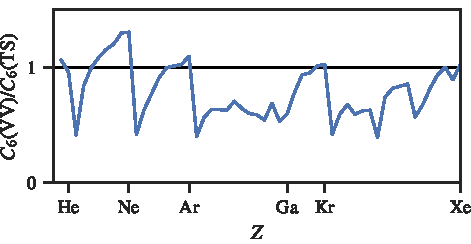
\includegraphics{../media/vv-periodic-table.pdf}
\caption{\textbf{Relative errors in VV polarizabilities of free atoms for first 54 elements.}
The reference values are the same as used in the TS method.
}\label{fig:vv-periodic-table}
\end{figure}

The VV polarizability functional is only approximate, which is manifest already for free-atom polarizabilities and $C_6$ coefficients, where accurate reference values are known (Figure~\ref{fig:vv-periodic-table}).
Whereas the VV functional reproduces atoms of nonmetallic elements quite accurately (especially the important carbon atom with error in the $C_6$ coefficient less than 2\%), the polarizabilities and $C_6$ coefficients of atoms of metallic elements are substantially underestimated.
To mitigate this error, we normalize the VV atomic quantities with the ratio of the free-atom polarizabilities and $C_6$ coefficients as calculated by the VV functional and as obtained from accurate reference calculations,
\begin{equation}
  \alpha_{0,i}^\text{rVV$'$}=\alpha_{0,i}^\mathrm{VV'}\frac{\alpha_{0,i}^\text{ref,free}}{\alpha_{0,i}^\text{VV$'$,free}},\quad
  C_{6,i}^\text{rVV$'$}=C_{6,i}^\mathrm{VV'}\frac{C_{6,i}^\text{ref,free}}{C_{6,i}^\text{VV$'$,free}}
\end{equation}
This correction assumes that any error in the VV functional is at least partially transferable from free atoms to atoms in compounds.
Alternatively, the normalization can be seen as a modification of the TS approach~\citep{TkatchenkoPRL09}, in which the ratios of Hirshfeld volumes are replaced with ratios of VV polarizabilities and $C_6$ coefficients.

% TODO
% As part of the normalization, we reoptimize the $C$ parameter in the VV functional on the same set of $C_6$ coefficients used in the TS method.
% The original formulation of the VV polarizability functional used $C=0.0089$~\citep{VydrovPRL09}, but was later reparametrized by the authors themselves to $C=0.0093$~\citep{VydrovJCP10a}.
% In both cases, the reference sets of $C_6$ coefficients used for the parametrization contained also atoms of metallic elements, which are severely underestimated by the VV functional (Figure~\ref{fig:vv-periodic-table}), and this pushed the parameter $C$ to lower values.
% The TS reference set contains mostly organic compounds, and this results in the higher value of $C=0.0101$.
% This makes the metallic elements even more underestimated by the VV functional, but that is not an issue in our approach because of to the normalization to free atoms.

% Jellium normalization {{{2

Many exchange--correlation (XC) functionals are exact for jellium by construction, even though the portion of electron correlation coming from plasmons is long-ranged and should not in principle be accounted for by semilocal XC functionals.
As a result of this construction, most XC functionals describe accurately the electron correlation \emph{within} slowly-varying density regions, such as those found in metals, and no addition of vdW forces is needed in those cases.
This is unlike in all other cases, where semilocal functionals neglect long-range vdW interactions.
Furthermore, the interactions \emph{between} such regions and other regions of the electron density are effectively screened by the conducting electrons.
At the same time, these metallic-density regions contribute dominantly to the polarizability in the VV functional (in principle the local polarizability of a conductor should be infinite) and hence to the vdW energy in any vdW model, in which the VV functional would be used directly.
When combined with semilocal DFT, this would result in overpolarization and overbinding of bulk metals as well as of adsorbates on metallic surfaces.
To avoid this double-counting of the long-range electron correlation, the VV10 expression for the vdW energy subtracts the limit of the VV10 nonlocal functional as the density gradient approaches zero, such that the vdW energy is equal to zero for jellium,
\begin{equation}
  E_\text{vdW}^\text{VV10} = E^\text{VV10}[n]-\bigl(E^\text{VV10}|_{\boldsymbol\nabla n\rightarrow0}\bigr)[n]
\end{equation}
Such an approach cannot be used directly in a many-body model such as MBD, because unlike in a pairwise model the many-body vdW energy is not linear in the polarizability.
This would result in all the nonlinear contributions, which can be dominating in a highly polarizable system such as a metal, not being subtracted by the zero-gradient limit.
Instead, we devised an alternative construction.

Rather than evaluating the interaction of the metallic-density regions and than subtracting it, as in VV10, we do not evaluate it in the first place by smoothly cutting of the contribution of these regions to the polarizability.
These regions can be distinguished using the combination of two local dimensionless electron-density descriptors: the local ionization potential $I$~\citep{GutleIJQC99} and the iso-orbital indicator $\chi$~\citep{BeckeJCP90,KummelMP03,SunPRL13},
\begin{equation}
  I[n]=\tau^\text{W}[n]/n,\qquad
  \chi[n]=\frac{\tau^\text{KS}[n]-\tau^\text{W}[n]}{\tau^\text{unif}[n]}
\end{equation}
where $\tau[n]=\sum_i|\boldsymbol\nabla\phi_i|^2/2$ is the positive kinetic energy density of occupied orbitals $\phi_i$, which for single-orbital densities reduces to the von Weizsäcker kinetic energy density, $\tau^\text W[n]=|\boldsymbol\nabla n|^2/8n$, and for jellium to $\tau^\mathrm{unif}[n]=3(3\pi^2)^{2/3}n^{5/3}/10$.  % chktex 3
The local ionization potential is a form of reduced gradient with the units of energy, which attempts to model the local electronic gap.
The density gradient alone is not sufficient to characterize metallic density.
In particular, both $I\sim0$ and $\chi\sim1$ must be true for density to be metallic, whereas $I\sim0$ and $\chi\sim0$ corresponds to centers of covalent bonds (dominated by a single bonding orbital) and $I\sim0$ and $\chi\gg1$ signifies overlaps of electron-density tails that occur between noncovalently bound systems.
Since the normalization of VV10 to jellium uses only the density gradient, it partially omits also contributions from covalent bonds.
By using the iso-orbital indicator, we can make MBD-NL more precise in this regard.

\begin{figure}[t!]
\begin{tikzpicture}
\node[below right] at (0,0) {\bfseries a};
\node[below right, inner sep=0pt] at (0,0) {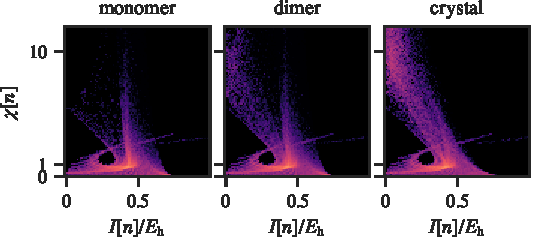
\includegraphics{../media/benzene.pdf}};
\node[below right] at (0,-4.3) {\bfseries b};
\node[below right, inner sep=0pt] at (0,-4.3) {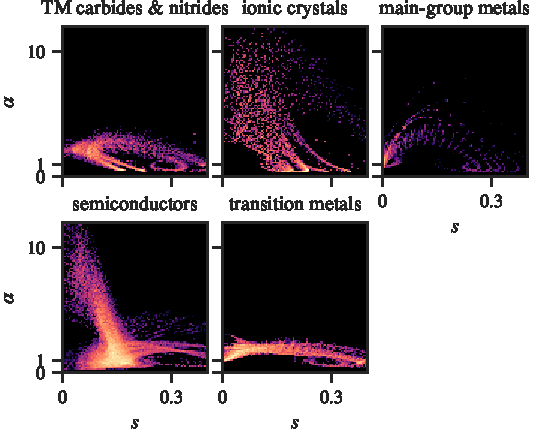
\includegraphics{../media/solids-hists.pdf}};
\end{tikzpicture}
\caption{\textbf{Polarizability distributions of local ionization potential $I$ and iso-orbital indicator $\chi$.}
Precisely, the plotted distributions are $\alpha^\text{VV}(s',\chi')=\int\mathrm d\mathbf r\delta(s(\mathbf r)-s')\delta(\chi(\mathbf r)-\chi')\alpha^\text{VV}(\mathbf r)$ such that the total polarizability is equal to $\iint\mathrm ds\mathrm d\chi\,\alpha^\text{VV}(s,\chi)$.
(\textbf a) Benzene monomer, dimer, and crystal.
Each distribution is normalized to one benzene molecule.
(\textbf b) 63 simple solids divided to five groups (see Supplementary Material for details).
Each distribution is normalized to 62 (a.\,u.), the VV polarizability of a benzene monomer, to share a single color scale with \textbf{a}.
}\label{fig:pol-hists}
\end{figure}

Figure~\ref{fig:pol-hists}a presents polarizability distributions of $I$ and $\chi$ in benzene compounds and in a set of simple solids, and shows that they are very sensitive to the nature of the bonding in a molecule or material.
In an organic molecule such as benzene (Figure~\ref{fig:pol-hists}a), the vast majority of the polarizability
comes from electron density with $I>\SI{5}{\electronvolt}$ while the small remainder comes
from low-gradient regions with $\chi<1$.
With the introduction of intermolecular interactions in the benzene dimer and crystal, a significant additional amount of polarizability comes from regions with $\chi\gg1$, despite the electron density being low in such regions.
A richer spectrum of patterns can be found in simple solids (Figure~\ref{fig:pol-hists}b).
Most similar to the benzene compounds is the group of semiconductors.
In contrast, the vast majority of the polarizability in main-group metals comes from jellium-like regions near $(I,\chi)=(0,1)$, as expected.
In transition metals, the polarizability is distributed over a wider range of the local gap along the $1<\chi<2$ strip, with a larger part still coming from low-gradient regions.
These features are largely shared by the transition-metal carbides and nitrides, but notably the near neighborhood of $(I,\chi)=(0,1)$ does not contribute in those systems.
In simple ionic solids, which do not feature covalent bonds, most of the polarizability comes from single-orbital regions ($\chi<1$), although a significant amount also comes from noncovalent orbital-overlap regions.

To avoid the double-counting of vdW interactions of low-gradient density regions, we smoothly cut off their contribution to the polarizability functional.
\begin{equation}
  \alpha^\mathrm{VV'}[n](\mathbf r)=g(I,\chi)\alpha^\text{VV}[n]
\end{equation}
We impose two simple requirements on this cutoff.
First, the density regions with a local gap lower than the work function of jellium ($<\SI{5}{\electronvolt}$) should not contribute to the calculated vdW energy.
Second, the VV polarizability of simple covalent compounds (exemplified by a benzene molecule) should not be influenced by the cutoff.
The following function $g$ satisfies these requirements:
\begin{gather}
  g(I,\chi)=1-\frac{1-f\bigl(\chi-3\sqrt{I}\bigr)}{1+\exp\bigl(4(I-\SI{5}{\electronvolt})/\SI{1}{\electronvolt}\bigr)}, \\
  f(x)=\exp\bigl(-cx/(1-x)\bigr)\theta(1-x)
\end{gather}
Function $g$ is composed from a logistic damping function centered at $\SI{5}{\electronvolt}$ with the width of $\SI{1}{\electronvolt}$, and form function $f$ taken from the SCAN functional~\citep{SunPRL15}, where it also serves to interpolate between $\chi=0$ and $\chi=1$.
We find that $c=0.1$ ensures that the effect of the cutoff on the VV polarizability of a benzene molecule is negligible ($<2\%$).

\begin{figure}[t!]
\centering
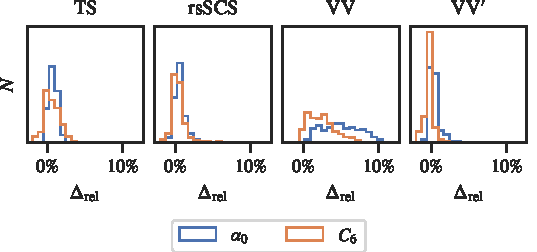
\includegraphics{../media/pol-shifts.pdf}
\caption{\textbf{Distributions of relative changes in atomic polarizabilities and $C_6$ coefficients from monomers to dimers.}
The distributions are calculated over all atoms from all complexes in the S66 data set.
}\label{fig:pol-shifts}
\end{figure}

Apart from avoiding the double-counting of long-range electron correlation in low-gradient regions, the cutoff function removes another deficiency of the VV polarizability functional.
When molecules are brought together to form vdW-bound compounds, the introduction of density-tail overlaps significantly increases the polarizability when using a model such as the VV functional (Figure~\ref{fig:pol-hists}a).
For instance, the VV polarizability per molecule goes from 62 (a.\,u.) in benzene monomer, to 67 in benzene dimer, to 92 in benzene crystal.
This effect is an artifact of the VV functional that causes increasingly large vdW-bound systems to be overbound, and cutting off the polarizability of low-gradient regions with $\chi>1$ eliminates this issue without
affecting the polarizabilities of isolated monomers compounds (Figure~\ref{fig:pol-shifts}).

% Many-body dispersion {{{2

The static polarizabilities and $C_6$ coefficients calculated as described above are put into the MBD model to obtain the vdW energy.
The MBD Hamiltonian describes a system of charges in harmonic potentials---Drude oscillators---characterized by their static polarizabilities $\alpha_{0,i}$ and resonance frequencies $\omega_i=4C_{6,ii}/3\alpha_{0,i}^2$, and interacting via a long-range dipole potential $\mathbf T^\mathrm{lr}(\mathbf R)\equiv f_\text{lr}(R)\mathbf T(\mathbf R)$,
\begin{multline}
  H^\text{MBD}(\{\alpha_{0,i},\omega_i\})=\sum_i-\frac12\nabla_{\xi_i}^2+\sum_i\frac12\omega_i^2\xi_i^2 \\
  +\frac12\sum_{ij}\omega_i\omega_j\sqrt{\alpha_{0,i}\alpha_{0,j}}\boldsymbol{\xi}_i\cdot\mathbf T^\mathrm{lr}_{ij}\boldsymbol{\xi}_j
\end{multline}
where $\boldsymbol\xi_i\equiv\sqrt{m_i}\mathbf x_i$ are mass-weighted displacements of the charges.
The interaction energy of this model system---the vdW energy---is readily obtained by direct diagonalization of the Hamiltonian in the basis of coupled oscillations with corresponding coupled frequencies $\tilde\omega_k$,
\begin{equation}
  E_\text{MBD}=\sum_k^{3N}\frac{\tilde\omega_k}2-\sum_i^N\frac{3\omega_i}2
\end{equation}

In MBD-NL, we use the same form of the long-range coupling $\mathbf T^\text{lr}$ as the MBD@rsSCS variant~\citep{AmbrosettiJCP14}, but with a different definition of the vdW radii.
Rather than using tabulated free-atom vdW radii, we use the simple formula for a vdW radius of \citet{FedorovPRL18}, and rather than with ratios of Hirshfeld volumes, these free-atom vdW radii are scaled with the ratios of VV polarizability of an atom in a compound and that of a free atom,\begin{equation}
  R_i^\text{vdW}=\tfrac52{(\alpha_{0,i}^\text{ref,free})}^\frac17{\left(\frac{\alpha_i^\mathrm{VV'}}{\alpha_i^\text{VV$'$,free}}\right)}^\frac13
\end{equation}
We reparametrize the damping parameter $\beta$ of $f_\text{lr}$ on the S66 data set and find the optimal values of 0.81 and 0.83 for the XC functionals PBE and PBE0, respectively, only slightly smaller than the optimal values of 0.83 and 0.85 of the MBD@rsSCS method.

% Tests {{{1

\begin{figure}[t!]
\centering
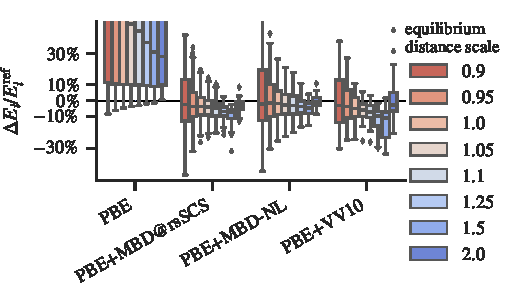
\includegraphics{../media/s66-errors.pdf}
\caption{\textbf{Distributions of relative errors in binding energies on the S66$\times$8 set of organic dimers.}
The scale encoded by the color multiplies the equilibrium distance between the centers of mass of two given monomers.
}\label{fig:s66-errors}
\end{figure}

\begin{figure}[t!]
\centering
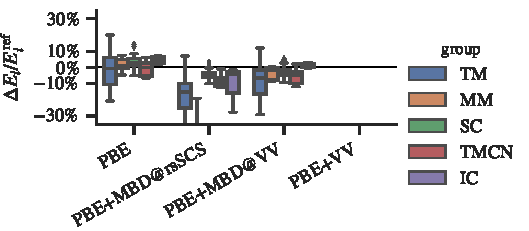
\includegraphics{../media/solids-errors.pdf}
\caption{\textbf{Distributions of relative errors in lattice energies on the set of 63 solids.}
The color encodes the class of a solid: transition metals (TM), main-group metals (MM), semiconductors (SC), transition-metal carbides and nitrides (TMCN), and ionic crystals (IC).
}\label{fig:solids-errors}
\end{figure}

\begin{table}[t!]
\centering
\caption{\textbf{Errors in interaction energies on vdW benchmark data sets.}}\label{tab:performance}
\small
\begin{tabular}{%
  ll
  *{2}{S[
    table-format=2.1,
    table-align-text-post=false,
    table-space-text-post=\%,
  ]}
  S[
    table-format=2.1,
    table-align-text-post=false,
  ]
  S[
    table-format=-2.1,
    table-align-text-pre=false,
    table-align-text-post=false,
    table-space-text-pre=k,
  ]
}
\toprule
method & & {S66} & {X23} & {S12L} & {``26''$^a$} \\
\midrule
PBE        & MRE$^b$  & 57\%   & 60\%   & 82\%   & 105\%      \\
+MBD@rsSCS & MARE$^c$ & 8.4\%  & 6.4\%  & 5.3\%  & (14\%)$^d$ \\
           & MRE      & -3.1\% & -3.4\% & -1.4\% & (-10\%)    \\
+MBD-NL    & MARE     & 9.3\%  & 6.2 \% & 9.2\%  & 21\%       \\
           & MRE      & -0.1\% & 1.9\%  & 6.4\%  & 21\%       \\
+VV10      & MARE     & 9.9\%  & 15\%   & 15\%   & (52\%)$^e$ \\
           & MRE      & -6.1\% & -15\%  & -15\%  & (-52\%)    \\
\midrule
PBE0       & MRE  & 56\%   & 58\%   & 75\%   & \\
+MBD@rsSCS & MARE & 7.6\%  & 5.4\%  & 6.5\%  & \\
           & MRE  & -1.1\% & -1.7\% & -4.4\% & \\
+MBD-NL    & MARE & 8.5 \% & 5.7\%  & 6.8\%  & \\
           & MRE  & 0.0\%  & 3.0\%  & 1.7\%  & \\
+VV10      & MARE & 8.3\%  & 15\%   & 20\%   & \\
           & MRE  & -5.3\% & -15\%  & -20\%  & \\
\bottomrule
\end{tabular}

\begin{minipage}{.96\linewidth}
\footenotesize%
$^a$Data set of interlayer binding energies of 26 layered materials with RPA benchmark energies by \citet{BjorkmanPRL12}.
$^b$Mean relative error. Negative numbers indicate overbinding.
$^c$Mean absolute relative error.
$^d$The eigenvalue rescaling for MBD by \citet{GouldJCTC16a} must be used, otherwise the MBD Hamiltonian has nonnegative eigenvalues for only 6 compounds (graphite, BN, PbO, and 3 TMDCs).
$^e$Results as given by \citet{BjorkmanPRB12} for the original PW86r+VV10 combination.
\end{minipage}
\end{table}

Next, we briefly describe several benchmark tests of the MBD-NL model, with details about the calculations, more detailed results, and additional tests reported in the Supplemental Material.
The performance on a set of small organic dimers (S66) is nearly identical to that of MBD@rsSCS (Figure~\ref{fig:s66-errors}), which is already excellent for a DFT+vdW approach.
In contrast, the errors in lattice energies of 63 simple solids are reduced drastically when MBD@rsSCS is replaced by MBD-NL (Figure~\ref{fig:solids-errors}).
This improvement comes mainly from the errors on metals and ionic solids, which PBE+MBD@rsSCS overbinds by tens of percent, whereas plain PBE performs reasonably well, and MBD-NL even slightly improves it.
PBE+MBD-NL still somewhat overbinds the metals compared to PBE, but this can be expected, because MBD-NL adds the nonlocal correlation between the bound nonconducting electrons of the metallic ions, which is missing in the PBE description, yet PBE does not underbind the metals.
The same holds for transition-metal carbides and nitrides.
Ionic solids are underbound by 4\% with PBE, which is reduced nearly to zero when the missing nonlocal correlation is added by MBD-NL, whereas MBD@rsSCS overbinds some of the ionic solids substantially.
The performance of MBD-NL on semiconductors is similar to that of MBD@rsSCS\@.

The overall performance on the S66 set, a set of organic molecular crystals (X23), a set of supramolecular complexes (S12L), and a set of 26 layered materials (``26'', \citet{BjorkmanPRB12}) is summarized in Table~\ref{tab:performance}.
On X23, the performance of MBD-NL is even slightly improved compared to MBD@rsSCS, with a similar tendency to underbind as that of MBD@rsSCS to overbind.
On S12L, the accuracy of PBE+MBD-NL is reduced compared to PBE+MBD@rsSCS, going from 5\% to 9\%, but the accuracy is equal with the PBE0 functional, with MBD-NL having a smaller MRE compared to MBD@rsSCS\@.
Of the three standard vdW data sets, S12L is the only one where PBE and PBE0 differ in performance.
This results mostly from PBE binding somewhat more the $\mathrm\pi$--$\mathrm\pi$ complexes.
The proper balance between semilocal DFT and long-range vdW models in the case of large $\mathrm\pi$--$\mathrm\pi$ complexes is unclear.

None of the existing DFT+vdW approaches, including the proposed MBD-NL, can properly describe the vdW interaction between two metallic systems, because that would require long-range coupling of the nonlocal metallic charge fluctuations, which none of these methods does.
In practice, this issue can be partially observed in layered vdW materials with small band gaps, such as the transition-metal dichalcogenides (TMDCs), which pose a hard problem for existing vdW methods.
TMDCs comprise 23 compounds in the ``26'' set of 26 layered materials compiled by \citet{BjorkmanPRL12}, besides hexagonal graphite and BN, and layered PbO, with reference energies obtained by random-phase approximation (RPA).
Both MBD@rsSCS and VV10 overbind the ``26'' set, by 10\% and 52\%, respectively, indicating that these models overpolarize the layered compounds (Table~\ref{tab:performance}).
This is further manifest in the fact that the MBD Hamiltonian has negative eigenvalues for 20 of the 26 compounds, which must be treated by the eigenvalue rescaling as proposed by \citet{GouldJCTC16a}.
The overpolarization is a result of both MBD@rsSCS and VV10 treating even the nonlocal part of the charge fluctuations in a local manner.
In contrast, this nonlocal part of the electronic response generated by low-gradient density regions is removed in the MBD-NL model, resulting in its underbinding of the ``26'' set by 21\%.
This is further corroborated by the fact that MBD-NL has the best accuracy from the three models for the three non-TMDC compounds in the ``26'' set (graphite, BN, PbO), with mean absolute relative error of 7\%, compared to 27\% (MBD@rsSCS) and 53\% (VV10).

\begin{figure}[t!]
\centering
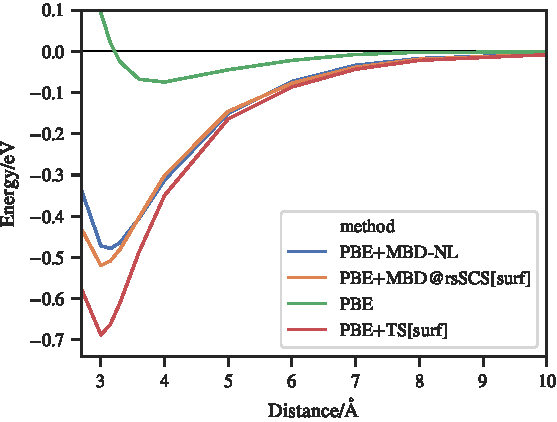
\includegraphics[width=\linewidth]{../media/surface.pdf}
\caption{\textbf{Binding energy of a single benzene molecule on a (111) silver surface.}
}\label{fig:silver-benzene}
\end{figure}

To complete a brief overview of the performance of the new model, we present a case relevant to surface science.
Figure~\label{fig:silver-benzene} shows the binding curve of a benzene molecule adsorbed on a (111) silver surface.
MBD-NL performs similarly to the MBD@rsSCS[surf] method~\citep{RuizPRB16}, which was developed specifically to treat adsorption of organic compounds on metallic surfaces, and provides accurate results compared to experiment.
The large relative magnitude of the many-body effects in this system can be seen from the comparison with the pairwise TS[surf] method.

% TODO discuss Gould

Before concluding, we discuss some of the potential weaknesses of MBD-NL\@.
First, the VV polarizability functional is semi-empirical and relatively simple, and its deficiencies can be observed already on the $C_6$ coefficients of free atoms (Figure~\ref{fig:vv-periodic-table}).
While we do correct for this by normalizing to free atoms, and the presented numerical results show a good accuracy on the studied systems, we expect that in general the VV functional is not able to capture in sufficient detail all electronic effects in polarizability that one can find either across chemical space or within a single class of compounds.
Second, although MBD-NL can effectively treat hybrid interfaces between organic and metallic compounds, it does not capture the truly nonlocal charge fluctuations that can be found in conductors~\cite{DobsonIJQC14}.
This limitation of using localized Drude oscillators is of lesser consequence in the hybrid interfaces, because the long-wavelength charge fluctuations in the metal do not have a correlation counterpart in the adsorbed organic compounds, but it would be manifest when studying vdW interactions between nano- or macroscopic metallic bodies.
Finally, as all other DFT+vdW approaches, MBD-NL uses an empirical range-separating function that needs to be parametrized for a given XC functional, and ensures that the electron correlation in the mid-range region is not double-counted.
While XC functionals such as PBE are usually well-behaved and the range separation is transferable across a broad spectrum of systems, the case of supramolecular $\mathrm\pi$--$\mathrm\pi$ complexes shows that this matter can not be entirely neglected.

In conclusion, we have developed a vdW model that combines advantages of interatomic many-body approaches and nonlocal pairwise functionals.
By normalizing to free atoms and jellium, we have retained the accuracy of best DFT+vdW approaches while extending applicability to ionic compounds and hybrid metal-organic interfaces, which is demonstrated by a number of benchmark calculations.
Our approach enables efficient, accurate, and consistent modeling of many-body vdW interactions in a substantially broader range of systems than previously possible.
